\documentclass{ximera}  

\title{Path Independence and FTLI}  

\begin{document}  
\begin{abstract}  
Fundamental Theorem of Line Integrals and path independence.
\end{abstract}  
\maketitle  

In the previous activity, we introduced some basic definitions from topology. These definitions are necessary in order to correctly state theorems in this section and the next, so pay attention to the hypotheses of these theorems!

We begin this activity by defining what it means for a vector field to be path independent. We then state and prove the Fundamental Theorem of Line Integrals. This theorem gives us an easy way to compute vector line integrals of a gradient field, provided the domain is open and connected. We then use the Fundamental Theorem of Line Integrals to show that conservative vector fields are path independent (under the appropriate conditions), and finish by discussing the various methods we now have for computing vector line integrals.

\section{Path Independence}

In this section, we introduce the idea of ``path independence'' for a vector field. We see an example of a vector field that is not path independent, and vector field that is path independent.

\begin{example}
Consider the vector field $\textbf{F}(x,y) = (y,0)$. Let $\textbf{x}(t)$ be the path from $(1,0)$ to $(0,1)$ along a straight line. Let $\textbf{y}(t)$ be the path from $(1,0)$ to $(0,1)$ counterclockwise around the unit circle. Compute $\int_\textbf{x} \textbf{F}\cdot d\textbf{s}$ and $\int_\textbf{y} \textbf{F}\cdot d\textbf{s}$. Are they equal?
\begin{explanation}
We'll begin by parametrizing our paths.
\[
\textbf{x}(t)= (\answer{1-t},\answer{t})\hspace{1cm}\textrm{for }t\in[0,1]
\]
\[
\textbf{y}(t)= (\answer{\cos(t)},\answer{\sin(t)})\hspace{1cm}\textrm{for }t\in[0,\frac{\pi}{2}]
\]
Now, we compute these line integrals using the definition
\[
\int_\textbf{x} \textbf{F}\cdot d\textbf{s} = \int_a^b\textbf{F}(\textbf{x}(t))\cdot \textbf{x}'(t)\,dt.
\]
Integrating along $\textbf{x}$, we have
\begin{align*}
\int_\textbf{x} \textbf{F}\cdot d\textbf{s} &= \int_a^b\textbf{F}(\textbf{x}(t))\cdot \textbf{x}'(t)\,dt\\
&= \int_{\answer{0}}^{\answer[given]{1}}(t,0)\cdot(-1, 1)\,dt\\
&= \int_{\answer{0}}^{\answer{1}}-t\,dt\\
&= \answer{-\frac{1}{2}}
\end{align*}
Integrating along $\textbf{y}$, we have
\begin{align*}
\int_\textbf{y} \textbf{F}\cdot d\textbf{s} &= \int_a^b\textbf{F}(\textbf{y}(t))\cdot \textbf{y}'(t)\,dt\\
&= \int_{0}^{\pi/2}(\sin(t),0)\cdot({\answer{-\sin(t)}}, {\answer{\cos(t)}})\,dt\\
&= \int_{0}^{\pi/2}\answer{-\sin^2(t)}\,dt\\
&= \answer{-\frac{\pi}{4}}
\end{align*}
Comparing $\int_\textbf{x} \textbf{F}\cdot d\textbf{s}$ and $\int_\textbf{y} \textbf{F}\cdot d\textbf{s}$, we see that they are
\begin{multipleChoice}
\choice{Equal.}
\choice[correct]{Not equal.}
\end{multipleChoice}
\end{explanation}
\end{example}

Now, let's investigate integrating a different vector field along those same paths.

\begin{example}
Consider the vector field $\textbf{F}(x,y) = (y,x)$. Let $\textbf{x}(t)$ be the path from $(1,0)$ to $(0,1)$ along a straight line. Let $\textbf{y}(t)$ be the path from $(1,0)$ to $(0,1)$ counterclockwise around the unit circle. Compute $\int_\textbf{x} \textbf{F}\cdot d\textbf{s}$ and $\int_\textbf{y} \textbf{F}\cdot d\textbf{s}$. Are they equal?
\begin{explanation}
Once again, we begin by parametrizing our paths.
\[
\textbf{x}(t)= (1-t,t)\hspace{1cm}\textrm{for }t\in[0,1]
\]
\[
\textbf{y}(t)= (\cos(t),\sin(t))\hspace{1cm}\textrm{for }t\in[0,\frac{\pi}{2}]
\]
Next, we compute these line integrals using the definition
\[
\int_\textbf{x} \textbf{F}\cdot d\textbf{s} = \int_a^b\textbf{F}(\textbf{x}(t))\cdot \textbf{x}'(t)\,dt.
\]
Integrating along $\textbf{x}$, we have
\begin{align*}
\int_\textbf{x} \textbf{F}\cdot d\textbf{s} &= \int_a^b\textbf{F}(\textbf{x}(t))\cdot \textbf{x}'(t)\,dt\\
&= \int_{0}^{1}(\answer{t},\answer{1-t})\cdot(-1, 1)\,dt\\
&= \int_{0}^{1}\answer{1-2t}\,dt\\
&= \answer{0}
\end{align*}
Integrating along $\textbf{y}$, we have
\begin{align*}
\int_\textbf{y} \textbf{F}\cdot d\textbf{s} &= \int_a^b\textbf{F}(\textbf{y}(t))\cdot \textbf{y}'(t)\,dt\\
&= \int_{0}^{\pi/2}(\answer{\sin(t)},\answer{\cos(t)})\cdot(-\sin(t), \cos(t))\,dt\\
&= \int_{0}^{\pi/2}\answer{-\sin^2(t)+\cos^2(t)}\,dt\\
&= \answer{0}
\end{align*}
Comparing $\int_\textbf{x} \textbf{F}\cdot d\textbf{s}$ and $\int_\textbf{y} \textbf{F}\cdot d\textbf{s}$, we see that they are
\begin{multipleChoice}
\choice[correct]{Equal.}
\choice{Not equal.}
\end{multipleChoice}
\end{explanation}
\end{example}

In fact, it turns out that if we integrate $\textbf{F}(x,y) = (y,x)$ along \emph{any} path starting at $(1,0)$ and ending at $(0,1)$, the integral will be $0$. So, the integral does not depend on the path we take to get between these two points. A vector field with this property is called \emph{path independent}.

\begin{definition}
A continuous vector field is called \emph{path independent} if $\int_C \textbf{F}\cdot d\textbf{s}=\int_D \textbf{F}\cdot d\textbf{s}$ for any two simple, piecewise $C^1$, oriented curves $C$ and $D$ with the same start and end points.
\end{definition}

Let's review the meaning of the requirements on the curves $C$ and $D$.

A curve is \emph{simple} if it \wordChoice{\choice{isn't too ``bumpy.''}\choice[correct]{doesn't intersect itself, except the start and end point can be the same.}\choice{is smooth.}}

A curve is $C^1$ if it \wordChoice{\choice{is continuous.}\choice{is differentiable.}\choice[correct]{has continuous partial derivatives.}}

A curve is \emph{oriented} if it \wordChoice{\choice[correct]{has a specified direction.}\choice{knows which way is North.}}

Our next question is: how do we know if a vector field is path independent? Of course, it's impossible to check every line integral over every possible curve between any two points - we would never finish these computations! Instead, we need some theorems that give us conditions under which a vector field is path independent. Our first step towards these theorems is the Fundamental Theorem of Line Integrals.

\section{Fundamental Theorem of Line Integrals}

We now introduce the Fundamental Theorem of Line Integrals, which gives us a slick way to compute the integral of a gradient vector field over a piecewise $C^1$ curve. In particular, note the conditions on the domain $X$: it must be open and connected.

\begin{theorem}
\textbf{Fundamental Theorem of Line Integrals}

Let $f:X\subset \mathbb{R}^n\rightarrow \mathbb{R}$ be $C^1$, where $X$ is open and connected. Then if $C$ is any piecewise $C^1$ curve from $\textbf{A}$ to $\textbf{B}$, then
\[
\int_C\nabla f\cdot d\textbf{s} = f(\textbf{B})-f(\textbf{A})
\]
\end{theorem}

This should look vaguely familiar - it resembles the Fundamental Theorem of Calculus from single variable calculus, also called the evaluation theorem.

We now prove the Fundamental Theorem of Line Integrals in the special case where we have a \emph{simple} parametrization of the curve $C$.

\begin{proof}
Let $\textbf{x}(t)$ be a simple parametrization of $C$, where $t\in[a,b]$, $\textbf{x}(a)=\textbf{A}$, and $\textbf{x}(b)=\textbf{B}$ (so the starting point is $\textbf{A}$, and the ending point is $\textbf{B}$).

Then we compute the line integral as:
\[
\int_C\nabla f\cdot d\textbf{s} = \int_\textbf{x}\nabla f\cdot d\textbf{s}.
\]
By the definition, we can compute this line integral as
\[
\int_\textbf{x}\nabla f\cdot d\textbf{s} = \int_a^b \nabla f(\textbf{x}(t))\cdot\textbf{x}'(t)\,dt.
\]
The integrand here should look familiar from one of the multivariable versions of the chain rule - it's the derivative of $f(\textbf{x}(t))$. Making this replacement, we have
\[
\int_\textbf{x}\nabla f\cdot d\textbf{s} = \int_a^b \frac{d}{dt}(f(\textbf{x}(t)))\,dt.
\]
Now, we can apply the Fundamental Theorem of Calculus (from single variable) to evaluate this integral, since an antiderivative for the integrand will be given by $f(\textbf{x}(t))$. From this we obtain:
\begin{align*}
\int_\textbf{x}\nabla f\cdot d\textbf{s} &= (f(\textbf{x}(t)))\vert_a^b\\
&= f(\textbf{x}(b))-f(\textbf{x}(a))\\
&= f(\textbf{B})-f(\textbf{A})
\end{align*}
In the last step, we use that $\textbf{A}$ and $\textbf{B}$ are the start an end points of $\textbf{x}(t)$, respectively.

Thus, we have proven the Fundamental Theorem of Line Integrals (when we have a simple parametrization of the curve $C$).
\end{proof}

Before discussing how the Fundamental Theorem of Line Integrals relates to path independence, let's look at how this helps us compute integrals of gradient vector fields.

\begin{example}
Let $\textbf{F}(x,y)=(y,x)$. Observe that $\textbf{F}=\nabla f$, where $f(x,y)=xy$. Compute $\int_C\textbf{F}\cdot d\textbf{s}$ for the curve $C$ below, starting at $(0,1)$ and ending at $(1,0)$.
\begin{center}
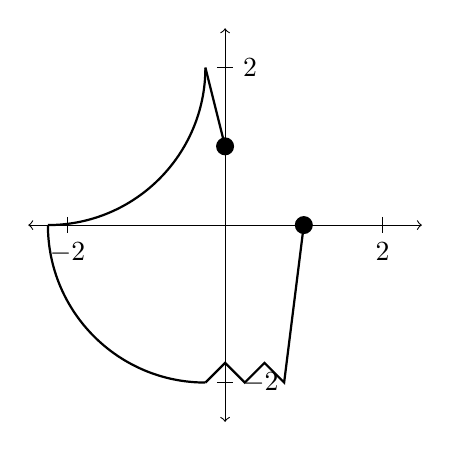
\begin{tikzpicture}
\draw[thick, fill=black] (1,0) circle (.1);
\draw[thick] (1,0) -- (0.75, -2) -- (0.5, -1.75) -- (0.25, -2) -- (0, -1.75) -- (-0.25, -2);
\draw[thick] (-0.25,-2) arc (270:180:2);
\draw[thick] (-2.25,0) arc (270:360:2);
\draw[thick] (-0.25,2) -- (0,1);
\draw[thick, fill=black] (0,1) circle (.1);

\draw[<->] (-2.5,0) -- (2.5,0);
\draw[<->] (0,-2.5) -- (0,2.5);
\foreach \x in {-2,2}
\draw[shift={(\x,0)},color=black] (0pt,3pt) -- (0pt,-3pt) node[below] 
{$\x$};
\foreach \y in {-2,2}
\draw[shift={(0,\y)},color=black] (-3pt,0pt) -- (3pt,0pt) node[right] 
{$\y$};
\end{tikzpicture}
\end{center}
\begin{explanation}
We certainly would like to avoid parametrizing this curve! So, we will use the Fundamental Theorem of Line Integrals to compute this integral.

First, let's verify that $\textbf{F}=\nabla f$ for $f(x,y)=xy$.
\begin{align*}
\frac{\partial}{\partial x}xy &= \answer{y}\\
\frac{\partial}{\partial y}xy &= \answer{x}
\end{align*}
Thus, we have $\nabla f(x,y)= (y,x) = \textbf{F}(x,y)$.

We can then use the Fundamental Theorem of Line Integrals to compute $\int_C\textbf{F}\cdot d\textbf{s}$.
\begin{align*}
\int_C\textbf{F}\cdot d\textbf{s} &= \int_C\nabla f\cdot d\textbf{s}\\
&= f(0,1) - f(1,0)\\
&= \answer{0}
\end{align*}

\end{explanation}
\end{example}

Now, it turns out that we can use the Fundamental Theorem of Line Integrals to prove the following corollary about the relationship between conservative vector fields and path independence. Note once again that we require the domain to be open and connected.

\begin{corollary}
If $\textbf{F}$ is a conservative vector field (so $\textbf{F}=\nabla f$ for some $f$) defined on an open and connected domain $X$, then $\textbf{F}$ is path independent.
\end{corollary}

\begin{proof}
Let $C$ and $D$ be two curves with starting point $\textbf{A}$ and ending point $\textbf{B}$. We will show that $\int_C\textbf{F}\cdot d\textbf{s}=\int_D\textbf{F}\cdot d\textbf{s}$.

Recall that ``$\textbf{F}$ is conservative'' means that $\textbf{F}=\nabla f$ for some function $f$, which will enable us to use the Fundamental Theorem of Line Integrals (FTLI). Then we have:
\begin{align*}
\int_C\textbf{F}\cdot d\textbf{s} &= \int_C\nabla f\cdot d\textbf{s}\\
&= f(\textbf{B})-f(\textbf{A})\hspace{1in}\textrm{(by FTLI)}\\
&= \int_D\nabla f\cdot d\textbf{s}\hspace{1in}\textrm{(also by FTLI)}\\
&= \int_D\textbf{F}\cdot d\textbf{s}.
\end{align*}
Thus, we have shown that $\int_C\textbf{F}\cdot d\textbf{s}=\int_D\textbf{F}\cdot d\textbf{s}$, and so have shown that $\textbf{F}$ is path independent.
\end{proof}

This corollary, with the Fundamental Theorem of Line Integrals, gives us a new tool for computing line integrals.

\section{Strategies for Computing Line Integrals}

We now have a few options for computing line integrals:

\begin{enumerate}
\item Using the original definition:
\[
\int_C\textbf{F}\cdot d\textbf{s} = \int_a^b\textbf{F}(\textbf{x}(t))\cdot \textbf{x}'(t)\,dt
\]
\item If $\textbf{F}$ is conservative (so $\textbf{F}=\nabla f$ for some $f$):
\begin{enumerate}
\item We can use the Fundamental Theorem of Line Integrals: 
\[
\int_C\textbf{F}\cdot d\textbf{s} = f(\textbf{B})-f(\textbf{A})
\]
\item Since the vector field is path independent, we can find an \emph{easier} path with the same start and end points, and integrate over that path.
\end{enumerate}
\end{enumerate}

Let's look at how these different methods can be used in an example.

\begin{example}
Let $\textbf{F}(x,y) = (2xy^2, 2x^2y)$, and consider $\textbf{x}(t)=(2\cos(\pi t),\sin(\pi t^2))$ for $t\in [0,1]$. Compute $\int_{\textbf{x}}\textbf{F}\cdot d\textbf{s}$.
\begin{explanation}
We'll evaluate this integral in three different ways.

First, let's evaluate using the definition of vector line integrals.
\begin{align*}
\int_{\textbf{x}}\textbf{F}\cdot d\textbf{s} &= \int_a^b\textbf{F}(\textbf{x}(t))\cdot \textbf{x}'(t)\,dt\\
&= \int_0^1(4\cos(\pi t)\sin^2(\pi t^2), 8\cos^2(\pi t)\sin(\pi t^2))\cdot (\answer{-2\pi\sin(\pi t)}, \answer{2\pi t\cos(\pi t^2)}\,dt\\
&= \int_0^1\answer{-8\pi\cos(\pi t)\sin(\pi t)\sin^2(\pi t^2) + 16\pi t\cos(\pi t^2)\cos^2(\pi t)\sin(\pi t^2)}\,dt
\end{align*}
This is an integral that it might be possible to figure out how to compute, but we certainly do not want to! We can use a computer algebra system to see that the result is $0$, but to compute the integral by hand, we will turn to our other methods.

For our alternate methods, we need to find a potential function $f(x,y)$ such that $\textbf{F}=\nabla f$. It turns out that $f(x,y)=x^2y^2$ works. Let's verify this.
\begin{align*}
\frac{\partial}{\partial x} (x^2y^2) &= \answer{2xy^2}\\
\frac{\partial}{\partial y} (x^2y^2) &= \answer{2x^2y}\\
\end{align*}

Now that we have our function $f(x,y)=x^2y^2$ such that $\textbf{F}=\nabla f$, we will use the Fundamental Theorem of Line Integrals to evaluate. Note the start and end points of our curve

\begin{align*}
\textbf{A} &= \textbf{x}(0) = (\answer{2}, \answer{0})\\
\textbf{B} &= \textbf{x}(1) = (\answer{-2}, \answer{0})\\
\end{align*}

\begin{align*}
\int_{\textbf{x}}\textbf{F}\cdot d\textbf{s} &= \int_{\textbf{x}}\nabla f\cdot d\textbf{s}\\
&= f(\textbf{B})-f(\textbf{A})\\
&= \answer{0}
\end{align*}

Note that this is a much easier computation than the integral we had from the first method.

Finally, we compute the line integral using the third method. We have already shown that $\mathbf{F}$ is a conservative vector field (by finding $f$ such that $\mathbf{F}=\nabla f$), and hence we know that $\mathbf{F}$ is path independent. So we can compute this integral by instead integrating over an easier path with the same start and end points, $(2,0)$ and $(-2,0)$, respectively. Let's choose the straight line from $(2,0)$ to $(-2,0)$, and parametrize this curve.
\[
\textbf{y}(t)=(\answer{t}, 0)\hspace{1cm} \textrm{for }t\in[-2,2]
\]
Now we can integrate over $y$ instead, which will be a much easier computation.
\begin{align*}
\int_{\textbf{x}}\textbf{F}\cdot d\textbf{s}  &= \int_{\textbf{y}}\textbf{F}\cdot d\textbf{s}\\
&= \int_{-2}^{2} \textbf{F}(\textbf{y}(t))\cdot \textbf{y}'(t)\,dt\\
&= \int_{-2}^{2} (\answer{0},\answer{0})\cdot (1,0)\,dt\\
&= \int_{-2}^{2} \answer{0}\,dt\\
&= \answer{0}
\end{align*}

So we've seen that we can compute this line integral in a few different ways, using the fact that the vector field is conservative.
\end{explanation}
\end{example}

Depending on the particular problem or example, any one of these methods might be easier than the others. You should practice trying these different methods, and see which you prefer! However, remember that for the second and third options, we need to first verify that the vector field $\mathbf{F}$ is conservative. This usually means finding a potential function $f$ such that $\mathbf{F}=\nabla f$.

\section{Summary}

In this activity, we introduced the following terms.
\begin{itemize}
\item Path independent
\end{itemize}
We also established the following results.
\begin{itemize}
\item The Fundamental Theorem of Line Integrals.
\item If $\textbf{F}$ is a conservative vector field defined on an open and connected domain $X$, then $\textbf{F}$ is path independent.
\end{itemize}

These results provide us with new methods to compute some vector line integrals.

In the next activity, we will discuss how we can determine whether or not a vector field is conservative.

\end{document}